% #############################################################################
% This is Chapter 6 - Research Proposal (the framework, as a method)
% !TEX root = ../main.tex
% #############################################################################
% SOURCE: docs/framework/Apex-Framework-v2.docx is the authoritative
% specification for this chapter. Its section numbering is preserved below so
% the two documents stay traceable to each other while writing.
% #############################################################################
\fancychapter{Research Proposal}
\label{chap:proposal}

This chapter presents the second and third activities of the \ac{DSRM}: the definition of objectives for a solution to the research problem formalised in \Cref{chap:problem}, and the design of the artefact that satisfies them, a process-oriented framework for governed Human-AI collaboration across the \ac{SDLC}. The framework is described here as a methodology, independently of any implementation; its instantiation as a working system is the subject of \Cref{chap:apex}.

% #############################################################################
\section{Objectives}
\label{sec:objectives}

The systematic literature review in \Cref{chap:slr} led to the problem formalised in \Cref{chap:problem}: the lack of structured guidance, methodological rigour and standardised evaluation practice for integrating these tools into development processes. The research objectives address that problem directly, and \Cref{tab:rq_objective_mapping} links each identified gap to the framework objective that resolves it.

{\footnotesize
\begin{longtable}{>{\raggedright\arraybackslash}p{0.6cm}
                  >{\raggedright\arraybackslash}p{5.0cm}
                  >{\raggedright\arraybackslash}p{3.0cm}
                  >{\raggedright\arraybackslash}p{5.0cm}}
\caption[Research questions, key findings, problem aspects and framework objectives]{Mapping between Research Questions, Key Findings, Problem Aspects, and Framework Objectives}
\label{tab:rq_objective_mapping} \\

% Header for the first page
\toprule
\textbf{RQ} & \textbf{Key Finding from SLR} & \textbf{Problem Aspect Addressed} & \textbf{Resulting Framework Objective} \\
\midrule
\endfirsthead

% Header for continuation pages
\toprule
\textbf{RQ} & \textbf{Key Finding from SLR} & \textbf{Problem Aspect Addressed} & \textbf{Resulting Framework Objective} \\
\midrule
\endhead

\midrule
\multicolumn{4}{r}{\textit{Continued on next page}}\\
\bottomrule
\endfoot

\bottomrule
\endlastfoot

RQ1 &
Usage is unevenly distributed across \ac{SDLC} phases and lacks structured integration. &
No structured guidance on where and how \ac{AI} should be applied across the \ac{SDLC}. &
Define a process framework mapping AI-supported activities to specific phases. \\ \addlinespace

RQ2 &
Recurring risks in reliability, validation, security and insufficient human oversight. &
Insufficient methodological support for risk, quality and accountability. &
Integrate governance mechanisms, human-in-the-loop practice and quality gates. \\ \addlinespace

RQ3 &
Significant variation among approaches and no consensus on managing adoption. &
Fragmentation of existing AI adoption methodologies. &
Consolidate practice into a unified, repeatable process-oriented framework. \\

\end{longtable}
}

% #############################################################################
\section{Purpose and Scope}
\label{sec:framework_scope}

% Framework doc §1. State plainly what the framework covers and what it does
% not. The exclusions matter: they pre-empt the "why is this not MLOps?"
% question from the committee.

The artefact is a method in the sense the \ac{DSRM} gives that term: phases, hats, artefacts and decision rules prescribing how a team organises the participation of \ac{AI} across the \ac{SDLC}. It is stated at the level of process rather than of tooling, so that it can be assessed independently of the system instantiating it in \Cref{chap:apex} and adopted against a different tool stack. It covers AI-assisted activity in every phase rather than the code-authoring phases alone, the collaboration and model-selection practices that activity requires, expressed as process obligations rather than a catalogue of prompts, and the governance mechanisms of \Cref{sec:governance}.

It excludes the training or fine-tuning of \acp{LLM}, model architecture design, \ac{MLOps} pipelines and tool-specific detail. These are boundaries rather than omissions, following from \Cref{chap:problem}'s concern with teams that \emph{consume} general-purpose models rather than \emph{produce} them: \ac{MLOps} governs a model's lifecycle as a deployed asset, while this framework governs the lifecycle of software a model helped write, and a pipeline can be mature under the first while the second remains ungoverned, which is the deficiency \Cref{chap:slr} reports. Tool-specific detail is excluded for the same reason \Cref{chap:apex,chap:evaluation} are kept separate: a framework prescribing a vendor cannot be evaluated independently of it.

% #############################################################################
\section{Design Principles}
\label{sec:design_principles}

% Framework doc §3. Each principle should be stated and then GROUNDED - the
% empirical citation is what separates this from an opinion piece, and it is
% the part an examiner will probe first.

Seven principles govern every subsequent design decision. Each is stated in \Cref{tab:principles} together with the evidence motivating it, since a principle asserted without grounding is a preference, and a framework built out of preferences cannot be defended as a research contribution. Where the grounding is a design commitment rather than an empirical finding, that is said so.

{\footnotesize
\begin{longtable}{>{\raggedright\arraybackslash}p{3.4cm}
                  >{\raggedright\arraybackslash}p{11.2cm}}
\caption{The seven design principles and the evidence grounding each}
\label{tab:principles} \\
\toprule
\textbf{Principle} & \textbf{Statement and grounding} \\
\midrule
\endfirsthead
\toprule
\textbf{Principle} & \textbf{Statement and grounding} \\
\midrule
\endhead

\midrule
\multicolumn{2}{r}{\textit{Continued on next page}}\\
\bottomrule
\endfoot

\bottomrule
\endlastfoot

Human-in-the-Loop by Design &
Every AI-generated artefact is subject to explicit human review and acceptance before entering the product. Adoption and trust diverge, at around 90\% daily use against roughly 30\% reporting low or no trust~\cite{DORA:2025ai}, and benchmarking shows the distrust warranted: the best agent and model combination was functionally correct 61\% of the time but secure only 10.5\%~\cite{Zhao:2025vibe}, and 45\% of samples across more than a hundred models introduced an OWASP Top 10 vulnerability, with security flat as correctness improved~\cite{Veracode:2025gen}. \\ \addlinespace

\ac{AI} as Augmentation, Not Substitution &
Humans retain responsibility for technical, architectural and quality decisions. In a randomised controlled trial developers took 19\% longer with assistance while estimating they had been 20\% faster~\cite{Becker:2025rct}; substituting judgement removes the only faculty able to notice such a discrepancy, and the \ac{SLR} reports reduced code understanding as a recurring consequence of unsupervised delegation~\cite{Banh:2025cf, Basha:2025tt, Jensen:2025me, Zamfiroiu:2025ec}. \\ \addlinespace

Process-Level Governance of \ac{AI} Usage &
AI participation is governed through repeatable mechanisms making contributions visible, traceable and attributable. \ac{AI} amplifies: capable teams become measurably more capable, dysfunctional teams measurably less so~\cite{DORA:2025ai}. If the surrounding process sets the sign of the effect, governance must live in the process rather than in prompt discipline. \\ \addlinespace

\ac{SDLC}-Wide and Phase-Aware Integration &
Participation is defined per phase, with hats and controls adapted to that phase's risks. Usage is unevenly distributed and concentrated on code generation, leaving requirements, design and maintenance with little guidance~\cite{Ahmed:2025ai, Hou:2025cl, Zhang:2025ea}; governing only the well-served phases would reproduce the gap the framework exists to close. \\ \addlinespace

Functional, Not Positional, Accountability &
Every role named is a function that must be performed, not a person who must exist, and for each AI-assisted activity a named hat, not a named person, is accountable for initiation, validation and acceptance. The structural half is a design commitment rather than an empirical claim, argued in \Cref{sec:roles}; its visible consequence is that no role is named whose only content is oversight. The accountability half follows from it directly: when an artefact has no identifiable author no party is answerable for its defects, and ownership is among the concerns most frequently raised by practitioners and organisations~\cite{Ahmed:2025ai, Banh:2025cf}. Accountability attaches to a function so that it survives the absence of any individual. \\ \addlinespace

Risk-Proportional Validation and Control &
Validation rigour is proportional to potential technical, organisational and ethical risk. The defect profile is not uniform: vulnerability rates reach 72\% for Java against 45\% overall and cluster in specific weakness categories~\cite{Veracode:2025gen, Zhao:2025vibe}. A uniform control is either too costly for the routine case or too weak for the dangerous one, which is why remediation separates a Fast Lane from a Secure Lane. \\ \addlinespace

Spec-Anchored Continuity &
A persistent versioned specification is maintained alongside the codebase and is what every AI-assisted activity is constrained by and validated against. As established in \Cref{sec:background_sdd} this instantiates spec-driven development rather than inventing it~\cite{Thoughtworks:2025SD, Farrag:2026sd}. The limitation belongs with the claim: its own principal source describes the practice as emerging and its scaling behaviour as an open risk~\cite{Thoughtworks:2025SD}, which \Cref{chap:evaluation} treats as something to test rather than assume. \\

\end{longtable}
}

% #############################################################################
\section{Lifecycle Phases and the AI Interaction Mapping}
\label{sec:phases}

% Framework doc §4-§5. This section answers DRQ1. The phase table (input,
% output, human responsibility, required controls, literature grounding) is the
% single most important artefact in this chapter - build it as a full-width
% table or a landscape page.

This section answers \ac{DRQ}1. The framework organises the lifecycle into six phases, preceded by a Strategic Alignment stage that sits outside the lifecycle proper because it is performed before the Squad is engaged at all: it decides whether a Unit of Work should exist, whereas the six phases decide how one is built. The six are Discovery and Requirements; Design, Prototyping and Architecture; Implementation; Testing; Deployment; and Maintenance. \Cref{tab:phase_mapping} fixes, for the stage and each of them, what enters, what the model is permitted to produce, what leaves, which hat is accountable, and which control must be satisfied before exit. It is the central artefact of this chapter and is not restated in prose.

Two mechanisms the table names are defined here, since both recur throughout the chapter. The \textbf{Interactive Bridge} is the interaction pattern governing Discovery and Requirements: the model drafts scenarios in plain natural language for human critique, the Trio confirms, adds, deletes or modifies them, and only the approved result is compiled into formal Gherkin and anchored. Separating critique from compilation matters because natural language is the medium in which a domain expert can detect a wrong assumption, whereas formal syntax invites review of the syntax instead. The \textbf{Consistency Factor} is the strict automated test set produced before generation begins, derived from both the functional and the technical specification, constraining what the model may produce rather than assessing it afterwards; it is specified in full in \Cref{sec:bolts}.

The framework's most direct precedent is the \ac{AI-DLC} published by Amazon Web Services~\cite{AWS:2025aidlc}, which organises work into Inception, Construction and Operations, replaces sprints with \emph{Bolts}, short cycles measured in hours or days, replaces Epics with \emph{Units of Work}, and governs AI participation through collaborative rituals of which \emph{Mob Elaboration} is adopted here; these three terms are taken directly from \ac{AI-DLC} with no originality claimed for them; its reported ten-to-fifteen-fold productivity improvement is vendor-reported, unreplicated and not carried here as evidence, adopted only as process vocabulary. Most of the expansion from three phases to six is decomposition rather than disagreement, since Discovery and Requirements together with Design, Prototyping and Architecture occupy the territory it calls Inception, and Implementation corresponds to Construction. Two extensions are substantive.

\noindent\textbf{The first is a decoupled Testing phase.} In \ac{AI-DLC}, build and test close Construction, performed in the same cycle by the same participants that generated the code. The objection is circularity, not thoroughness: tests derived by the same model, from the same specification, encode the same reading of the requirement as the implementation, so passing them confirms internal consistency rather than external correctness. Benchmark evidence shows exactly this asymmetry: agent-generated code passes functional tests far more often than independently held security tests, and the gap does not close as models improve~\cite{Zhao:2025vibe, Veracode:2025gen}. Testing therefore becomes its own phase, with its own environment, hat and gate, working from the locked functional specification rather than the implementation; the unit of validation changes at this boundary, from the Bolt's task to the assembled User Story, the smallest unit at which business value is observable.

\noindent\textbf{The second is a distinct Maintenance phase with a diagnostic firewall.} \ac{AI-DLC}'s Operations phase is deployment with monitoring, defining no mechanism for classifying post-deployment signals or routing them to an owner. The signal is heterogeneous, a defect against an agreed specification, a request never specified, or evidence the specification was wrong, and treating all three as defects erodes the specification, each undocumented accommodation widening the gap between what the system does and what the record says it should. A signal is therefore classified before any code is opened, and Context Reconstruction limits the developer to the specific report, the test evidence and the isolated fragment implicated, prohibiting whole-project context, a control for the reason developed in \Cref{sec:spec_anchored}~\cite{Zhao:2025vibe}.

The phases are listed in an order, but that order is not the shape of the process: Maintenance neither terminates the lifecycle nor patches in place. Its exit is always an entry into a named earlier phase, whose gate then applies in full: a business deviation routes to the \ac{PM} hat for a value decision and, if approved, re-opens Discovery and Requirements; a specification gap re-opens Design, Prototyping and Architecture with the technical specification amended and re-versioned; a production defect re-enters Implementation as a Fix-Bolt and returns through Testing. This is not Waterfall with a maintenance tail: in Waterfall, feedback is measured against a specification treated as frozen, whereas here the specification is exactly what is re-opened, re-approved and re-versioned, and code is regenerated from it. What the framework refuses is the unnamed loop, a change applied to production code with no corresponding change to the specification it is supposed to satisfy, since that is how traceability is lost in practice. \Cref{fig:lifecycle} shows the six phases and these three loop-backs; \Cref{tab:phase_mapping} is the detail behind each box.

\begin{figure}[htbp]
    \centering
    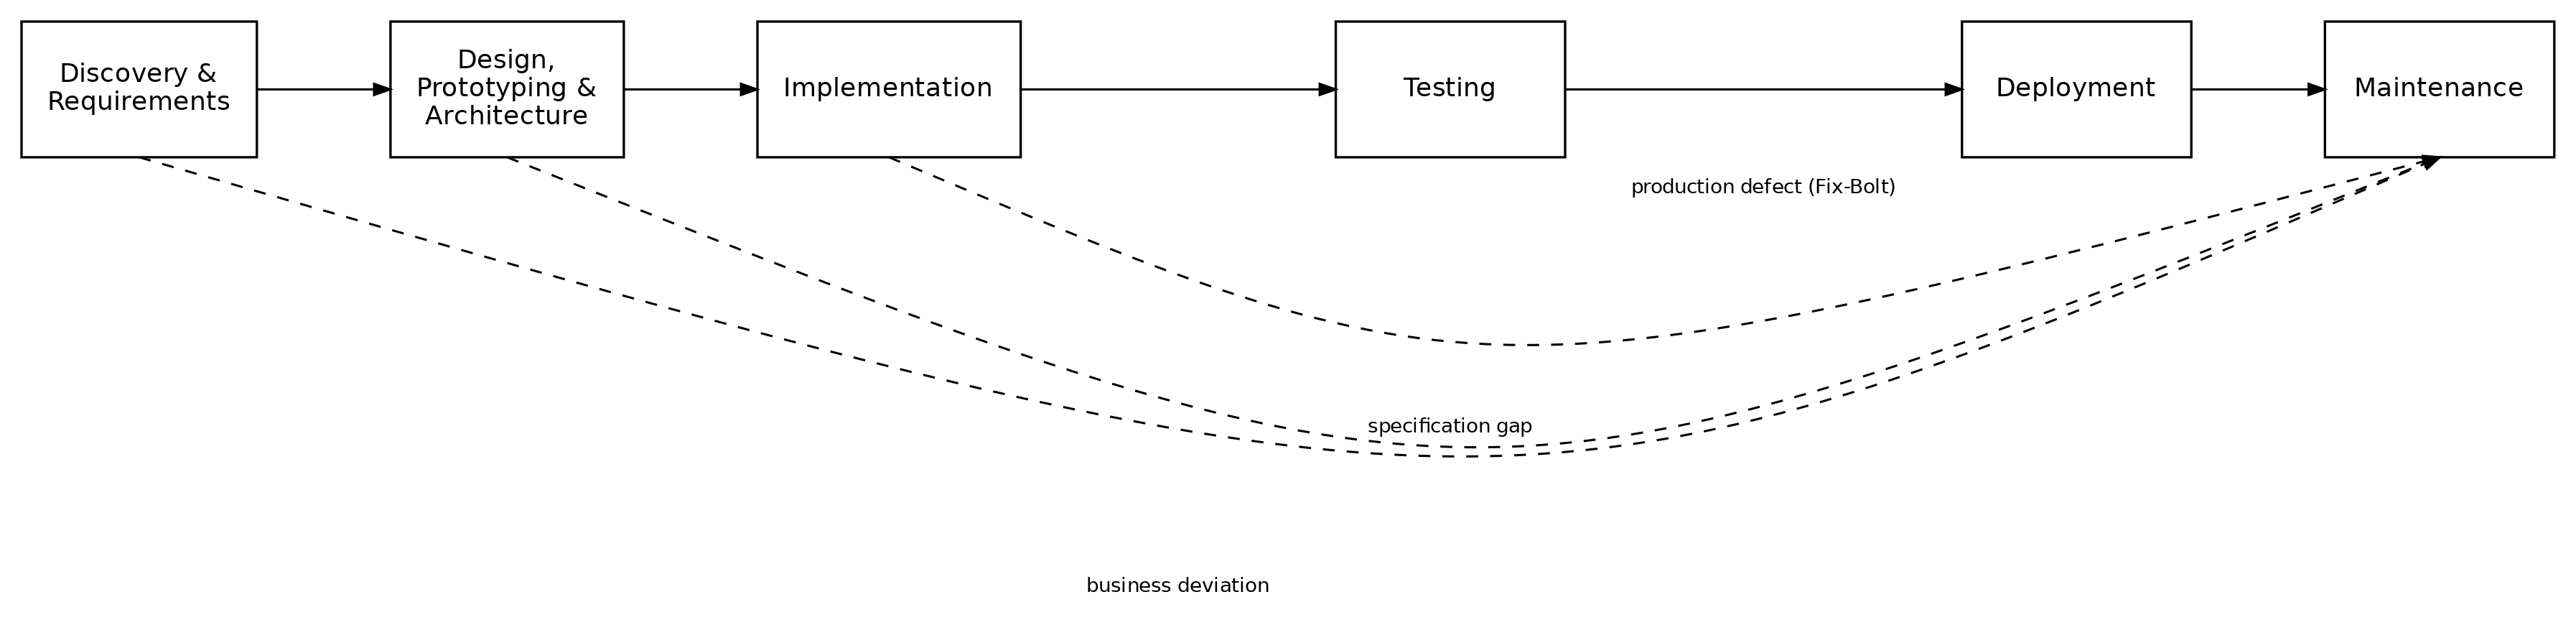
\includegraphics[width=\linewidth]{./Images/lifecycle-diagram.png}
    \caption[The six lifecycle phases and the three loop-backs out of Maintenance]{The six lifecycle phases in sequence, and the three named loop-backs out of Maintenance. Each loop-back re-enters a specific earlier phase, whose gate then applies in full - Maintenance never patches production code without a corresponding change to the specification.}
    \label{fig:lifecycle}
\end{figure}

{\scriptsize
\renewcommand{\arraystretch}{1.3}
\setlength{\tabcolsep}{4pt}
\begin{longtable}{>{\raggedright\arraybackslash}p{1.95cm}
                  >{\raggedright\arraybackslash}p{3.25cm}
                  >{\raggedright\arraybackslash}p{2.85cm}
                  >{\raggedright\arraybackslash}p{3.25cm}
                  >{\raggedright\arraybackslash}p{3.2cm}}
\caption[The six lifecycle phases and the preceding Strategic Alignment stage]{The six lifecycle phases and the preceding Strategic Alignment stage: permitted AI contribution, output, accountable hat, and the control that must be satisfied before each is exited. Each phase takes as input the output of the one above it.}
\label{tab:phase_mapping} \\

\toprule
\textbf{Phase} & \textbf{Role of AI} & \textbf{Output} & \textbf{Human accountability} & \textbf{Mandatory control} \\
\midrule
\endfirsthead

\toprule
\textbf{Phase} & \textbf{Role of AI} & \textbf{Output} & \textbf{Human accountability} & \textbf{Mandatory control} \\
\midrule
\endhead

\midrule
\multicolumn{5}{r}{\textit{Continued on next page}}\\
\bottomrule
\endfoot

\bottomrule
\endlastfoot

Strategic Alignment (pre-lifecycle) &
Assists market analysis; drafts candidate objectives and indicators &
A Unit of Work carrying a stated business justification, \acp{OKR} and \acp{KPI} &
\ac{PM} hat aligns the product vision with stakeholders and owns the justification &
Stakeholder alignment and \ac{OKR} sign-off before the Unit of Work reaches the Squad \\
\midrule

Discovery \& Requirements &
Drafts fractional User Stories in natural language; compiles approved scenarios into formal Gherkin &
Approved User Stories sized XS or S, with Gherkin acceptance criteria and stable scenario identifiers &
The Trio validates correctness, completeness and business value through the Interactive Bridge &
Mob Elaboration and the Discovery Gate \\
\midrule

Design, Prototyping \& Architecture &
Proposes architectural options; generates \ac{UI} structure and a formal technical specification &
Approved prototype and an anchored technical specification (interface contract, data model, runtime contract) &
Design Lead hat validates usability; Tech Lead hat validates feasibility, scalability and integration risk &
Design Gate; no task enters the Bolt Backlog until both validations pass \\
\midrule

Implementation &
Generates and refactors code constrained by the Consistency Factor test set &
Task-level code passing the pipeline and the Consistency Factor &
Developer hat validates output, owns correctness and security, and must be able to explain the logic &
Pre-Bolt architectural lock, the Bolt micro-cycle, and the Implementation Gate at story level \\
\midrule

Testing &
Drafts end-to-end \ac{BDD} scripts derived from the approved Gherkin &
A story-level verdict and, on failure, the exact failing evidence &
\ac{QA} hat verifies and refines generated scripts before execution and probes edge cases manually &
The \ac{QA} Validation Playbook and the Testing Gate, in a separate environment decoupled from the Bolt \\
\midrule

Deployment &
Answers the infrastructure delta question; generates configuration, \ac{IaC} or migrations only when required &
A released increment and a persistent context updated to the live state &
Whoever performs the deployment approves it and reviews its security implications &
Deployment Gate, performed by the deploying hat; no separate gatekeeping team is assumed \\
\midrule

Maintenance &
Reconstructs a deliberately narrow context to explain one specific failure and proposes a bounded fix &
A classified signal routed to the phase that owns it, with a verified diagnosis where applicable &
Developer or \ac{PM} hat classifies the signal and must verify any diagnosis before it is trusted &
Diagnostic firewall (Context Reconstruction, whole-project context prohibited) and governed loop-back to a named phase \\

\end{longtable}
}


% #############################################################################
\section{Roles and Responsibilities}
\label{sec:roles}

% Framework doc §6. The "hats, not people" framing is a deliberate design
% decision and should be argued as one, not merely asserted.

Every role named is a hat: a function the framework requires to be performed, not a person who must be hired. One individual may wear several hats, and on a small team a hat may go unfilled, its responsibility falling to whoever performs the adjacent work. \Cref{tab:hats} summarises the hats and the gate each owns. Three reasons justify expressing responsibility as a function rather than a position: it fits a target population of anyone with a technical background working alone or in a small team, whom a staffed-organisation role model would exclude; accountability expressed as a title lapses the moment the title is vacant, whereas a function survives reassignment; and the third is evidential, concerning what happens when structural models are copied as blueprints.

The Trio, comprising the \ac{PO}, Tech Lead and Design Lead hats, is inspired by the Squad concept popularised in the Spotify Model, and citing that model honestly requires citing its limits alongside it. It was published as a description of one company at one point in time, not a method for adoption elsewhere~\cite{Kniberg:2012sp}, its own principal author has since called it inspiration rather than a blueprint~\cite{LeadingComplexity:2023sp}, and a former employee's first-hand account names two failure modes never resolved internally: unclear matrix decision authority, and autonomy without accountability~\cite{Lee:2020sq}. The framework hardens against exactly these two. Matrix ambiguity is answered by the Tech Lead hat's architectural lock, fixing the technical boundary before any Bolt begins; autonomy without accountability is answered by separating logistics authority in the Bolt Master hat from technical authority in the Tech Lead hat, with every gate attached to a named function. A closer structural match is Team Topologies' stream-aligned team, which treats cognitive load as an explicit design constraint~\cite{Skelton:2019tt}: limiting developer agency over scope during a Bolt reduces the open decisions held while validating generated code, the activity \Cref{sec:motivation} identifies as the new constraint. The \ac{PM} hat, sitting outside the Squad, is structurally closer to the single-threaded leader Amazon adopted after its two-pizza structure stopped surviving scale~\cite{Bryar:2021wb}.

Deployment approval and infrastructure-security review are mandatory, but owned by whoever performs the deployment, self-reviewed solo or peer-reviewed where a second developer exists, rather than by an external DevOps Alliance: naming a governance function without naming who holds it is the defect explicit responsibility exists to prevent, since a body defined only by what it supervises can be assumed by the process to exist and never actually staffed.

The gates do not relax as the team shrinks. On a solo project each gate is self-checked, but what it requires is unchanged: the evidence in \Cref{tab:gates} must exist, be recorded, and be examined deliberately at the moment the gate is reached, not assumed to have been examined during the work that produced it. A gate's value lies primarily in forcing an explicit, separate act of validation against a written specification that predates the artefact, which is what makes self-review meaningful even when the reviewer and the author are the same person.

{\footnotesize
\begin{longtable}{>{\raggedright\arraybackslash}p{2.4cm}
                  >{\raggedright\arraybackslash}p{8.6cm}
                  >{\raggedright\arraybackslash}p{3.6cm}}
\caption{The hats: the function each discharges and the gate each owns}
\label{tab:hats} \\
\toprule
\textbf{Hat} & \textbf{Function the framework requires} & \textbf{Gate owned} \\
\midrule
\endfirsthead
\toprule
\textbf{Hat} & \textbf{Function the framework requires} & \textbf{Gate owned} \\
\midrule
\endhead

\midrule
\multicolumn{3}{r}{\textit{Continued on next page}}\\
\bottomrule
\endfoot

\bottomrule
\endlastfoot

\ac{PM} & Stakeholder alignment, \acp{OKR} and \acp{KPI}, and the business justification of a Unit of Work before it reaches the Squad; receives classified business deviations from Maintenance. & Strategic alignment sign-off \\ \addlinespace
\ac{PO} (Trio) & Business value and prioritisation of User Stories; leads the critique of AI-drafted scenarios during Mob Elaboration. & Discovery, with the Trio \\ \addlinespace
Tech Lead (Trio) & Technical specification, architectural feasibility and integration risk; decomposes stories into tasks and flags high-risk ones before any Bolt begins. & Design (technical) and the pre-Bolt architectural lock \\ \addlinespace
Design Lead (Trio) & Prototype or visual element for every feature, and its validation through usability testing. & Design (usability) \\ \addlinespace
Bolt Master & Continuous flow: prioritises the Bolt Backlog, manages dependencies, assigns by capacity once the Tech Lead hat has approved. & None; holds logistics authority deliberately separated from technical authority \\ \addlinespace
Developer & Executes tasks with the model, generates and validates the Consistency Factor, and remains answerable for correctness, security and being able to explain the logic. & Implementation \\ \addlinespace
\ac{QA} & Validates the assembled story against the approved Gherkin in a separate environment, verifying generated \ac{BDD} scripts before execution and probing edge cases manually. & Testing \\ \addlinespace
Deploying hat & Not a distinct role: whoever performs a release approves it and reviews the security of any generated \ac{IaC} or configuration. & Deployment \\

\end{longtable}
}

% #############################################################################
\section{Governance Mechanisms and Quality Gates}
\label{sec:governance}

% Framework doc §7. This section answers DRQ2 and is the core contribution.

\subsection{Bolts as the Unit of Execution}
\label{sec:bolts}
A Bolt is the smallest execution iteration the framework recognises: the implementation of one task within a User Story, strictly inside the development environment and measured in hours rather than weeks. The term is adopted from \ac{AI-DLC}~\cite{AWS:2025aidlc}; what the framework adds is the sequence of obligations around it, since a short cycle without a fixed reference is a fast way to accumulate divergence.

Before any code is generated, the Tech Lead hat feeds the locked context (the approved Gherkin, the prototype and the technical specification) to the model, verifies the task list it proposes, and flags high-risk tasks. This \textbf{architectural lock} makes the technical boundary a matter of record rather than negotiation, letting tasks on either side of an interface proceed in parallel. The Bolt Master hat then assigns by capacity, giving developers the story's intent, not authority over the technical scope the lock has settled. A Developer hat pulls one task, at which moment the Bolt begins and Bolt Cycle Time is measured from. Developer and model then produce the \textbf{Consistency Factor}, a strict automated test set derived from both specifications that constrains generation rather than reporting on it afterwards; the model generates against that constraint and the developer refines the result as an active editor, not an approver of a finished proposal. A task is done when the code passes the pipeline \emph{and} the developer can explain the logic, since code no one can explain has been substituted for engineering rather than added to it. When every task is done, the story passes the Implementation Gate into staging.

The \textbf{Fix-Bolt} is the single exception: triggered by a failed Testing Gate or a verified defect, it omits task breakdown because the context already contains what that step would produce, the exact failing scenario and its evidence. It is justified by what is already known rather than being a licence to skip planning for a change that merely feels small. Its outcome is routed by risk, where the risk-proportional principle becomes operational: a low-risk patch takes the \textbf{Fast Lane} directly to the delivery pipeline without re-entering formal \ac{QA}, while a higher-risk one takes the \textbf{Secure Lane} back to staging for a Regression Bypass, in which \ac{QA} re-runs the existing suite before verifying the targeted patch.

\subsection{Spec-Anchored Continuity}
\label{sec:spec_anchored}
Spec-Anchored Continuity requires every AI-generated artefact to carry forward the context established by previously validated phases. The mechanism is a persistent versioned specification maintained alongside the codebase and split into two layers with different lifetimes. The \textbf{global layer}, the Memory Bank, holds what does not change between stories: architectural rules, technology-stack decisions, security policies and recorded workarounds for already-diagnosed defects. It is written rarely, amended deliberately, and applies to every generation on the project. The \textbf{local layer}, the Feature Specs, holds what is specific to the work in hand, the approved Gherkin acceptance criteria and the technical specification produced at the Design Gate; it is written once per story, locked at a gate, and amended only through a recorded versioned amendment. The split is what makes the mechanism usable, since a single undifferentiated context grows monotonically until it contains more irrelevant material than relevant, reintroducing the problem it was meant to solve.

The central argument is that narrowing the model's working context is a control rather than a convenience: a convenience makes a correct outcome easier to reach, whereas a control is a measure whose absence makes an incorrect outcome undetectable. Anchoring satisfies the second definition on three counts. It supplies a reference that existed before the generated artefact did, the precondition for validation being possible at all. It bounds what the model may act upon, an unbounded context being the condition under which a model produces a wide, confident and substantively wrong change, which is why whole-project context is prohibited during Maintenance diagnosis~\cite{Zhao:2025vibe}. And because both layers are versioned and every post-lock edit is a dated amendment, divergence between what was agreed and what was built becomes a detectable event rather than an unattributable drift. This is the spec-driven-development instantiation named in \Cref{tab:principles}; a recent preprint independently argues, from a multivocal review, that specification discipline rather than model capability is the binding constraint on dependability~\cite{Farrag:2026sd}. The contribution is not the idea of anchoring but the specification of where it is mandatory, which gate locks each layer, and what constitutes a legitimate amendment.

\subsection{Quality Gates}
\label{sec:gates}
A quality gate has three named components: an owning hat, a specific body of evidence that must exist and be examined, and a defined consequence when it is absent or inadequate. A checkpoint missing any of the three is a ceremony rather than a control, since it can be passed without anything being established. \Cref{tab:gates} specifies the five gates on those terms. Notably, failure never discards work and never silently degrades it, but returns it to a named earlier activity with the evidence attached, the same routing discipline Maintenance applies to post-deployment signals.

{\footnotesize
\begin{longtable}{>{\raggedright\arraybackslash}p{1.9cm}
                  >{\raggedright\arraybackslash}p{2.1cm}
                  >{\raggedright\arraybackslash}p{5.2cm}
                  >{\raggedright\arraybackslash}p{5.0cm}}
\caption{The five quality gates: owner, required evidence, and the consequence of failure}
\label{tab:gates} \\
\toprule
\textbf{Gate} & \textbf{Owning hat} & \textbf{Evidence required to pass} & \textbf{Consequence of failure} \\
\midrule
\endfirsthead
\toprule
\textbf{Gate} & \textbf{Owning hat} & \textbf{Evidence required to pass} & \textbf{Consequence of failure} \\
\midrule
\endhead

\midrule
\multicolumn{4}{r}{\textit{Continued on next page}}\\
\bottomrule
\endfoot

\bottomrule
\endlastfoot

Discovery & The Trio & Testable Gherkin acceptance criteria approved through the Interactive Bridge; every story sized XS or S; the functional specification locked and versioned. & Scenarios return to Mob Elaboration; oversized stories are decomposed before re-submission. \\ \addlinespace
Design & Design Lead and Tech Lead hats & An approved prototype validated by usability testing; a technical specification covering interface contract, data model and runtime contract, anchored into the persistent context. & Feedback returns to prototype generation or architectural specification; no task may enter the Bolt Backlog. \\ \addlinespace
Implementation & Developer hat & Every task complete, passing the pipeline and the Consistency Factor, with the developer able to explain the generated logic. & The story does not enter staging; incomplete or unexplained tasks return to the Bolt Backlog. \\ \addlinespace
Testing & \ac{QA} hat & The assembled story validated in staging against the locked Gherkin through verified \ac{BDD} scripts, with edge cases probed manually. & A Fix-Bolt is triggered with the exact failing evidence attached; the story re-enters staging afterwards. \\ \addlinespace
Deployment & Whoever performs the deployment & Explicit approval of the release and a security review of any generated \ac{IaC}, configuration or migration; the persistent context updated to the live state. & The specific objection is fed back for a compliant regeneration; the release does not proceed. \\

\end{longtable}
}

\subsection{Governance Metrics}
\label{sec:metrics}
Three governance metrics are defined, chosen to measure whether the collaboration is safe and whether it is flowing rather than to measure output volume, the quantity \Cref{sec:motivation} shows rising without a corresponding improvement in delivery~\cite{Faros:2025par}. \textbf{Bolt Cycle Time} is the elapsed time from a task being pulled as a Bolt to its being marked done, defined at task level rather than story level because a story-level measurement conflates execution with the queueing, review and gate transitions surrounding it, and the claim about continuous flow is a claim about execution. \textbf{Context Traceability Rate} is the proportion of deployed Bolts and stories whose context chain is complete, the deployed artefact resolving back to a locked technical specification, to the functional specification it derived from, and to the Unit of Work that motivated it; it measures whether Spec-Anchored Continuity is holding in practice rather than merely being prescribed. \textbf{AI Defect Escape Rate} is the proportion of production defects originating in AI-generated logic that passed the Testing Gate, and it is the metric that detects a gate which has become ceremonial, since a gate satisfied without being exercised shows up here and nowhere else.

These are expressed in vocabulary continuous with established \ac{AI} governance standards rather than bespoke to this work: the \ac{NIST} \ac{AI} Risk Management Framework's Govern, Map, Measure and Manage~\cite{NIST:2023rmf} correspond respectively to this chapter's design principles, phase mapping, metrics and gates, and ISO/IEC 42001:2023 offers a complementary plan-do-check-act vocabulary for the same loop~\cite{ISO/IEC:2023ai}. This is a claim about shared language only: neither the framework nor Apex has been audited against either standard, and nothing here asserts compliance or intent to certify, only that these constructs occupy the conceptual space standards bodies are converging on.

% #############################################################################
\section{Work Organisation}
\label{sec:work_organisation}

% Framework doc §8. The argument for replacing sprint cadence must rest on the
% measured bottleneck shift, not on preference.

The framework replaces the familiar hierarchy of epics, sprints and sprint backlogs with continuous flow, the most disruptive single element of the proposal and therefore the one requiring the strongest empirical justification. Sprint cadence manages a world in which implementation is the binding constraint: a fixed-length iteration lets a quantity of implementation work be forecast, committed to and inspected at a boundary, calibrated to how long a useful amount of implementation takes. The evidence in \Cref{sec:motivation} indicates that premise no longer holds where AI assistance is heavy: developers in a randomised controlled trial were measurably slower with assistance while believing they had been faster~\cite{Becker:2025rct}, and telemetry across 1,255 teams pairs the merged-pull-request increase reported there with pull requests 154\% larger, 91\% longer review times, and no significant correlation with delivery outcomes~\cite{Faros:2025par}. The constraint moved rather than disappeared, so a cadence calibrated to the old one now obscures the new one. The structural response has two parts: execution compressed into Bolts, so the queue in front of validation refills in small increments rather than batches, and validation decoupled into its own phase, environment, hat and gate, so the constraint is scheduled and measured in its own right. Both are falsifiable: if review is not the constraint in a given setting, Bolt Cycle Time and the \ac{QA} queue will say so.

Three levels of work are retained, and the vocabulary of the upper two follows \ac{AI-DLC}~\cite{AWS:2025aidlc}. A \textbf{Unit of Work} is the core business problem, owned by the \ac{PM} and \ac{PO} hats, the level at which business justification is argued and acceptance criteria are generated as a group; grouping them this way rather than requirement by requirement is itself supported by evaluation, an epic-organised pipeline outperforming a requirement-aligned baseline across 107 requirements on expert-rated correctness (4.61 against 4.14 out of 5) and completeness (4.31 against 3.50)~\cite{Siddeeq:2026gh}. \textbf{User Stories} are the tangible deliverables, constrained to extra-small or small, the level at which \ac{QA} tests because they are the smallest unit at which business value is observable; the size constraint is load-bearing, since a story describable by a handful of scenarios is small enough for a reviewer to hold in mind while validating generated code against it. \textbf{Tasks} are the granular technical steps executed as Bolts, entering the \textbf{Bolt Backlog}, a continuous prioritised queue, only after decomposition with the model, Tech Lead verification, and risk flagging. Developers have limited agency over task creation and selection deliberately, not out of distrust: the decisions withheld are exactly those the architectural lock has settled, for the cognitive-load reason argued in \Cref{sec:roles}. The team's project management tool is expected to expose states corresponding to the phases as guidance rather than a literal requirement; what matters is that each column maps unambiguously onto one phase.

% #############################################################################
\section{Operational Playbooks}
\label{sec:playbooks}

% Framework doc §9. Six playbooks, each a step-by-step procedure. Presented as
% a single table rather than six algorithm environments, for length.

The phases, gates and hats state what must hold; the six playbooks in \Cref{tab:playbooks} state how the recurring procedures are performed, each with its trigger, its participants and its termination condition. A team that follows these six and observes the gates in \Cref{tab:gates} is operating the framework, irrespective of the tooling it uses. In Maintenance, the prohibition on whole-project context is the single most restrictive rule in the framework, for the reason given in \Cref{sec:phases}. In the Fix-Bolt, the Regression Bypass re-runs the existing \ac{BDD} suite rather than regenerating it, because a regenerated suite is a different measurement instrument, and comparing a patched system against it cannot distinguish a fixed defect from a changed test.

{\footnotesize
\begin{longtable}{>{\raggedright\arraybackslash}p{2.1cm}
                  >{\raggedright\arraybackslash}p{2.8cm}
                  >{\raggedright\arraybackslash}p{6.3cm}
                  >{\raggedright\arraybackslash}p{3.0cm}}
\caption{The six operational playbooks: trigger, procedure, and termination}
\label{tab:playbooks} \\
\toprule
\textbf{Playbook} & \textbf{Trigger} & \textbf{Procedure} & \textbf{Terminates when} \\
\midrule
\endfirsthead
\toprule
\textbf{Playbook} & \textbf{Trigger} & \textbf{Procedure} & \textbf{Terminates when} \\
\midrule
\endhead

\midrule
\multicolumn{4}{r}{\textit{Continued on next page}}\\
\bottomrule
\endfoot

\bottomrule
\endlastfoot

Mob Elaboration & A Unit of Work brought to the Squad & The Trio supplies intent, personas and domain constraints; the agent drafts fractional stories in natural language; the Trio cross-examines for value, feasibility and coherence, issuing confirm, add, delete or modify instructions until satisfied; the agent then compiles the approved scenarios into Gherkin and anchors the result. & The Discovery Gate passes and the functional specification is locked \\ \addlinespace

Design and Prototyping & Locked Gherkin acceptance criteria & The Design Lead hat prompts for screens and flows; the Tech Lead hat prompts for interface contract, data model and runtime contract and anchors them; usability testing and architectural review run in parallel. & Both validations pass and tasks enter the Bolt Backlog \\ \addlinespace

Maintenance and Evolution & A post-deployment signal & Classify before any code is opened: a business deviation or specification gap routes to the \ac{PM} hat for a value decision and re-opens the owning phase; a technical defect routes to a Developer hat, who narrows the context to the report, the test evidence and the isolated fragment, asks only why that logic failed, and verifies the diagnosis manually. & The signal is classified and routed, with a verified diagnosis where applicable \\ \addlinespace

Fix-Bolt & A failed Testing Gate or a verified defect & Pulled immediately with task breakdown skipped; the agent resolves only the specific defect while adhering to the anchored specification; the developer reviews for newly introduced vulnerabilities, not only symptom resolution; existing and new unit tests must pass. & Low risk takes the Fast Lane to the pipeline; higher risk takes the Secure Lane through a Regression Bypass in staging \\ \addlinespace

\ac{QA} Validation & A story that has passed the Implementation Gate & The \ac{QA} hat opens the locked functional specification rather than the implementation, prompts for end-to-end \ac{BDD} scripts and verifies them manually \emph{before} execution, since an unverified script can report a passing scenario it never exercised, then probes edge cases exploratively. & The Testing Gate passes, or a Fix-Bolt is triggered with the failing evidence \\ \addlinespace

Deployment and Release & A story that has passed the Testing Gate & The agent answers one bounded question, whether the release requires new infrastructure, configuration or migrations, and generates artefacts only when it does; whoever deploys reviews any generated artefact for vulnerabilities and policy violations. & The Deployment Gate passes and the persistent context is updated to the live state \\

\end{longtable}
}

% #############################################################################
\section{Positioning Against Alternatives}
\label{sec:alternatives}

% Framework doc §10. A design is only defensible against named alternatives.
% This section is what makes the artefact a research contribution rather than a
% proposal, and it is where a committee will press hardest.

A design is only defensible against named alternatives. Four are engaged below, each stated at its strongest, credited with what it genuinely does better, and met with the evidence motivating a different choice; the sources cited throughout ground individual pieces of an original synthesis, not a joint blueprint this work reproduces.

\begin{itemize}[leftmargin=0.6cm, itemsep=0.5em]

\item \textbf{No framework at all.} Premise: model capability suffices and process overhead is pure cost, correct for a short-lived prototype with no maintenance horizon, no coordination cost, no artefact to maintain, no gate to turn ceremonial. Documented failure mode, not hypothetical: \Cref{sec:design_principles} already establishes that functionally correct agent output is insecure at scale and that security does not improve as correctness does~\cite{Zhao:2025vibe, Veracode:2025gen}, so waiting is not a valid strategy. Flat, not merely lagging, is what turns validation from discipline into a structural requirement.

\item \textbf{Adopt \ac{AI-DLC} as published and unmodified.} Premise: a coherent three-phase model already exists from a credible source, and extending it adds complexity without control~\cite{AWS:2025aidlc}; genuinely simpler, operated at commercial scale, less process surface for a small team. The objection is narrow, the two gaps argued in \Cref{sec:phases}: build and test folded into the close of Construction, and an Operations phase with no published mechanism for classifying post-deployment feedback. The divergence fills gaps its own documentation leaves open; its vendor-reported, unverified productivity claims are not grounds to adopt it unmodified.

\item \textbf{Keep Scrum or SAFe cadence and treat \ac{AI} as a faster development environment.} Premise: existing ceremonies already provide planning, review and retrospection, and \ac{AI} only changes the speed of one activity; not trivial, since the cadence is understood, tooled, compatible with planning cycles, and costs nothing in retraining. \Cref{sec:work_organisation} already shows why that premise fails, pairing the same controlled-experiment and telemetry evidence: developers underestimate the slowdown assistance introduces~\cite{Becker:2025rct} while the constraint has moved from implementation to review~\cite{Faros:2025par}. The retrospective this alternative relies on to catch that is a weak instrument for catching it, and an iteration boundary calibrated to implementation keeps reporting on the activity that is no longer binding.

\item \textbf{Metrics-only governance, with no phase structure.} Premise: an organisation can track the right capabilities and outcomes, publish them, and let teams self-organise. The most serious of the four: far cheaper to adopt, presumes no lifecycle shape, adapts to context, and its own literature legitimately warns that no single metric can stand for the whole and any measure elevated to a target stops being a good one~\cite{Forsgren:2021sp}. The response is a distinction, not a rebuttal: metrics measure whether governance is working, they are not themselves a governance mechanism. A dashboard can accurately report rising review time and escaping defects while containing no mechanism for what a model may act upon, no point where an artefact must be checked against a prior specification, and no rule for where a post-deployment signal is routed, which is why the framework defines its own metrics in the same vocabulary rather than proposing an alternative to measurement.

\end{itemize}

% #############################################################################
\section{Summary}
\label{sec:proposal_summary}

\ac{DRQ}1 and \ac{DRQ}2 are answered by the artefact this chapter has specified: the six-phase model of \Cref{sec:phases} with the Strategic Alignment stage preceding it and the mapping in \Cref{tab:phase_mapping}, and \Cref{sec:governance}'s governance set of Bolts, the Consistency Factor, Spec-Anchored Continuity, five gates and three metrics. Two properties of that answer are worth isolating, because a phase list and a gate list alone would not achieve them: the model is constrained at every phase to that phase's anchored specification rather than the whole project, and accountability attaches to functions rather than positions, so it survives a team of one while every failed gate routes work back to a named phase rather than discarding it.

Both answers are design claims and not yet evidence. The framework's constructs are an original synthesis argued from the literature but not demonstrated in use, and spec-driven development, on which Spec-Anchored Continuity rests, is characterised by its own principal source as emerging with unsettled scaling behaviour~\cite{Thoughtworks:2025SD}. \Cref{chap:apex} presents Apex, the reference implementation, and reports which constructs were implementable as specified, which were weakened or proxied, and which resisted implementation, the substance of \ac{DRQ}3.
